\usetikzlibrary{arrows}
\usetikzlibrary{fit}

\tikzset{
	pics/conv/.style n args={5}{
		code = {
			\draw[draw=black] (#1, #2) rectangle ++ (1, 3) node[rotate=90, pos=0.5] {\large $#3 \times #4 \times #3$};
			\node[below] at (#1+0.5, #2+3.1) {\large #5};
		}
	},
	pics/text/.style n args={5}{
		code = {
			\draw[draw=black] (#1, #2) rectangle ++ (1, 3) node[rotate=#4, pos=0.5] {\huge #3};
			\node[below] at (#1+0.5, #2+3.1) {\large #5};
		}
	}
}

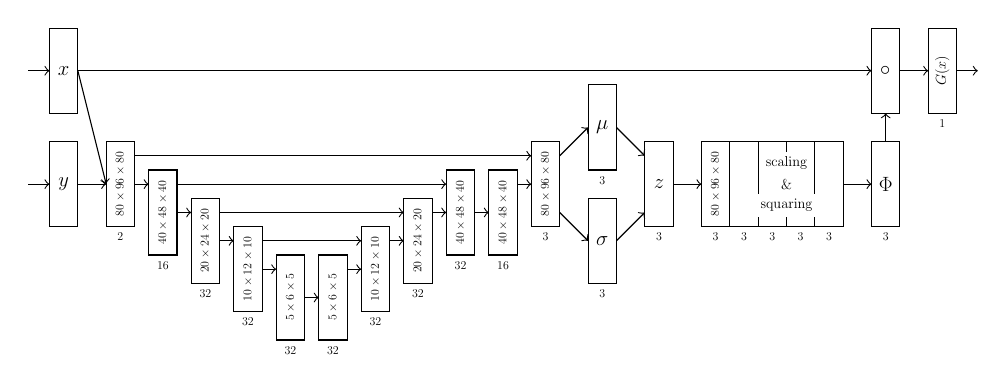
\begin{tikzpicture}[scale=0.36, line/.style={>=latex}, every node/.style={scale=0.36}, y=-1cm] 

	\pic{text={-2}		{0}	{$y$}	{0}	{}};
	\pic{text={-2}		{-4}	{$x$}	{0}	{}};

	\pic{conv={0}		{0}	{80}	{96}	{2}};
	\pic{conv={1.5}		{1}	{40}	{48}	{16}};
	\pic{conv={3}		{2}	{20}	{24}	{32}};
	\pic{conv={4.5}		{3}	{10}	{12}	{32}};
	\pic{conv={6}		{4}	{5}	{6}	{32}};
	\pic{conv={7.5}		{4}	{5}	{6}	{32}};
	\pic{conv={9}		{3}	{10}	{12}	{32}};
	\pic{conv={10.5}	{2}	{20}	{24}	{32}};
	\pic{conv={12}		{1}	{40}	{48}	{32}};
	\pic{conv={13.5}	{1}	{40}	{48}	{16}};
	\pic{conv={15}		{0}	{80}	{96}	{3}};
	
	\pic{text={17}		{-2}	{$\mu$}	{0}	{3}};
	\pic{text={17}		{2}	{$\sigma$}	{0}	{3}};
	
	\pic{text={19}		{0}	{$z$}	{0}	{3}};

	\pic{conv={21}		{0}	{80}	{96}	{3}};
	\pic{text={22}		{0}	{}	{0}	{3}};
	\pic{text={23}		{0}	{}	{0}	{3}};
	\pic{text={24}		{0}	{}	{0}	{3}};
	\pic{text={25}		{0}	{}	{0}	{3}};
	
    	\node [fill=white, inner sep=5pt] at (24, 0.75) {\Large scaling};
	\node [fill=white, inner sep=5pt] at (24, 1.5) {\Large \&};
    	\node [fill=white, inner sep=5pt] at (24, 2.25) {\Large squaring};

	\pic{text={27}	 	{0}	{$\Phi$}	{0}	{3}};
	
	\pic{text={27}		{-4}	{$\circ$}{90}	{}};
	
	\pic{text={29}		{-4}	{\Large $G(x)$}	{90}	{1}};

	\draw[->] (-2.75, -2.5) -- (-2, -2.5);
	\draw[->] (-2.75, 1.5) -- (-2, 1.5);
	\draw[->] (-1, 1.5) -- (0, 1.5);
	\draw[->] (-1, -2.5) -- (0, 1.5);

	\draw[->] (1, 1.5) -- (1.5, 1.5);
	\draw[->] (2.5, 2.5) -- (3, 2.5);
	\draw[->] (4, 3.5) -- (4.5, 3.5);
	\draw[->] (5.5, 4.5) -- (6, 4.5);
	\draw[->] (7, 5.5) -- (7.5, 5.5);
	\draw[->] (8.5, 4.5) -- (9, 4.5);
	\draw[->] (10, 3.5) -- (10.5, 3.5);
	\draw[->] (11.5, 2.5) -- (12, 2.5);
	\draw[->] (13, 2.5) -- (13.5, 2.5);
	\draw[->] (14.5, 1.5) -- (15, 1.5);

	% distribution
	\draw[->] (16, 0.5) -- (17, -0.5);
	\draw[->] (16, 2.5) -- (17,  3.5);

	\draw[->] (18, -0.5) -- (19,  0.5);
	\draw[->] (18, 3.5) -- (19,  2.5);
	
	\draw[->] (20, 1.5) -- (21,  1.5);
	
	\draw[->] (26, 1.5) -- (27,  1.5);

	\draw[->] (27.5, 0) -- (27.5, -1);
	
	\draw[->] (-1, -2.5) -- (27, -2.5);

	\draw[->] (28, -2.5) -- (29,  -2.5);
	\draw[->] (30, -2.5) -- (30.75, -2.5);

	% skip connections
	\draw[->] (1, 0.5) -- (15, 0.5);
	\draw[->] (2.5, 1.5) -- (12, 1.5);
	\draw[->] (4, 2.5) -- (10.5, 2.5);
	\draw[->] (5.5, 3.5) -- (9, 3.5);
	
	%\node [fill=white, inner sep=5pt] at (10.25, 2) {skip connections};

\end{tikzpicture}
